After implementing the verilog code.
We used the timing function to verify the working of the code.
Below, we are attaching the screenshots from the timing diagram

\begin{figure}[h]
    \begin{center}
        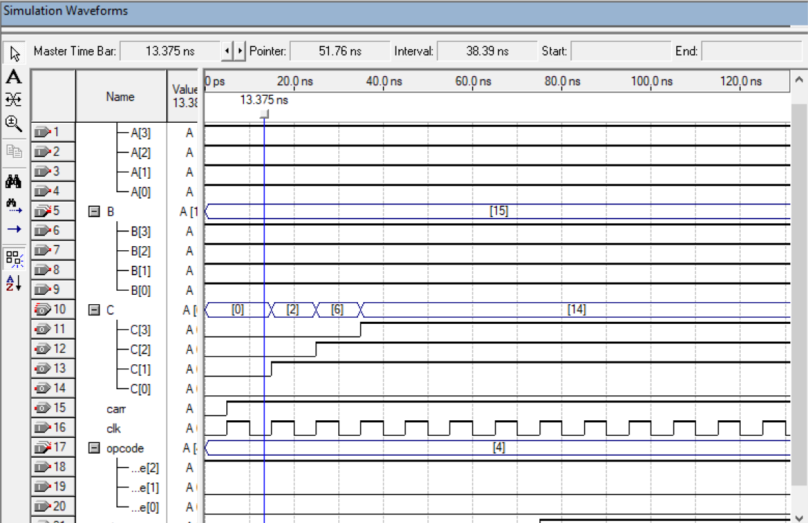
\includegraphics[scale=0.2]{figures/add}
    \end{center}
    \caption{Timing Daigram for ADD Operation}
    \label{fig:timing add}
\end{figure}

\begin{figure}[h]
    \begin{center}
        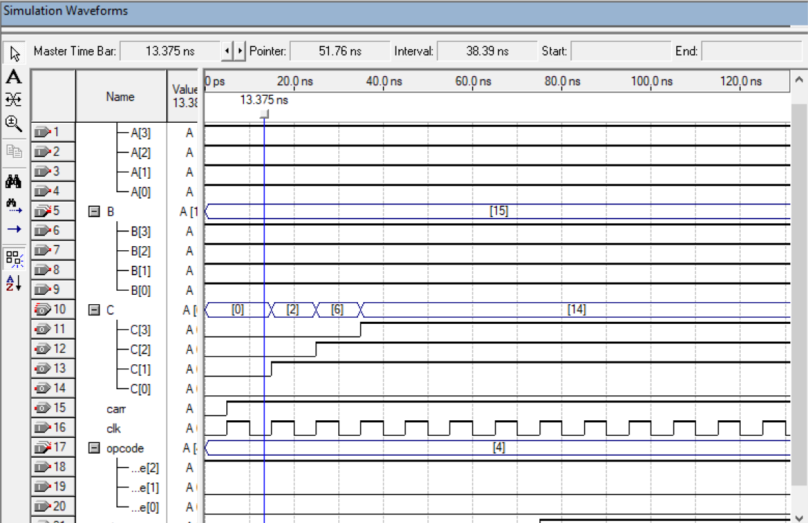
\includegraphics[scale=0.2]{figures/add}
    \end{center}
    \caption{Sub Operation does not work properly}
    \label{fig:timing sub}
\end{figure}

\begin{figure}[h]
    \begin{center}
        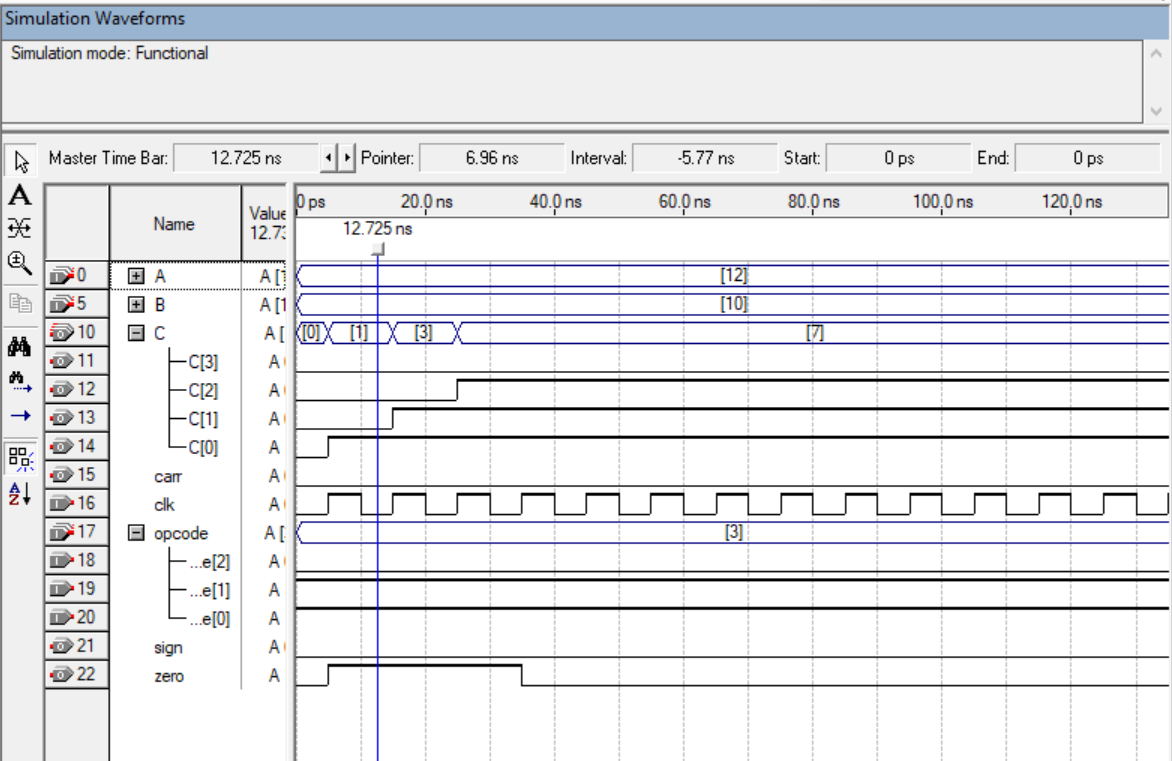
\includegraphics[scale=0.2]{figures/nand}
    \end{center}
    \caption{Timing Daigram for NAND Operation}
    \label{fig:timing nand}
\end{figure}

\begin{figure}[h]
    \begin{center}
        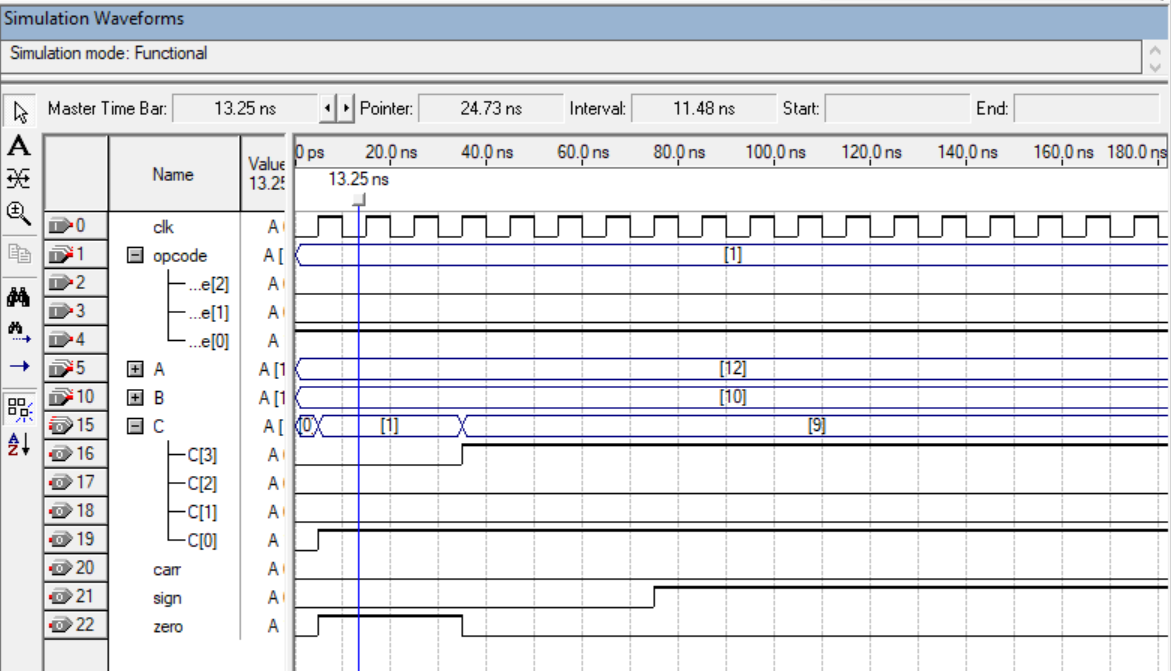
\includegraphics[scale=0.2]{figures/xnor}
    \end{center}
    \caption{Timing Daigram for XNOR Operation}
    \label{fig:timing xnor}
\end{figure}

\textbf{NAND} and \textbf{XNOR} operation are pretty much straight forward.
All we had to do is put the equation in the verilog and then the
operation performed as expected.
Below timing diagram, those operations are attached.
